\documentclass[a4paper,11pt]{article}
\usepackage[polish]{babel}
\usepackage[OT4]{fontenc}
\usepackage[utf8]{inputenc}
\usepackage{graphicx}
\usepackage{subfig}
\usepackage{epstopdf}




\date{21/03/2014}


%opening
\title{PAMSI -- testowanie algorytmów sortowania}
\author{Piotr Wilkosz}


\captionsetup{belowskip=12pt,aboveskip=4pt}
\begin{document}

\maketitle



\section{Wstęp}
Celem ćwiczenia było przetestowanie złożoności obliczeń algorytmów. Do testowania zostały wybrane 3 z puli algorytmów na ocenę bardzo dobrą:
\begin{itemize}
 \item Quick-sort (sortowanie szybkie)
 \item Heap-sort (sortowanie przez kopcowanie)
 \item Merge-sort (sortowanie przez scalanie)
\end{itemize}

\section{Wyniki pomiarów}

\begin{enumerate}
 \item Quick-sort - dane malejące:
   
  \begin{table}[th]
  \centering
    \caption{Pomiar czasu sortowania szybkiego dla danych posortowanych malejąco}

      \begin{tabular}{|l|l|l|}
	\hline
	N & czas & odchylenie \\
    \hline
 100 & 2.69796e-05 & 5.85553e-06\\
 \hline
1000 & 0.00162174 & 0.000156749\\
\hline
10000 & 0.159148 & 0.0182501\\
\hline
50000 & 3.88031 & 0.354078\\
\hline
100000 & 15.5052 & 1.40588\\


\hline
    \end{tabular}
    \label{tab1}
    \end{table}
 \begin{figure}[!h]
\centering
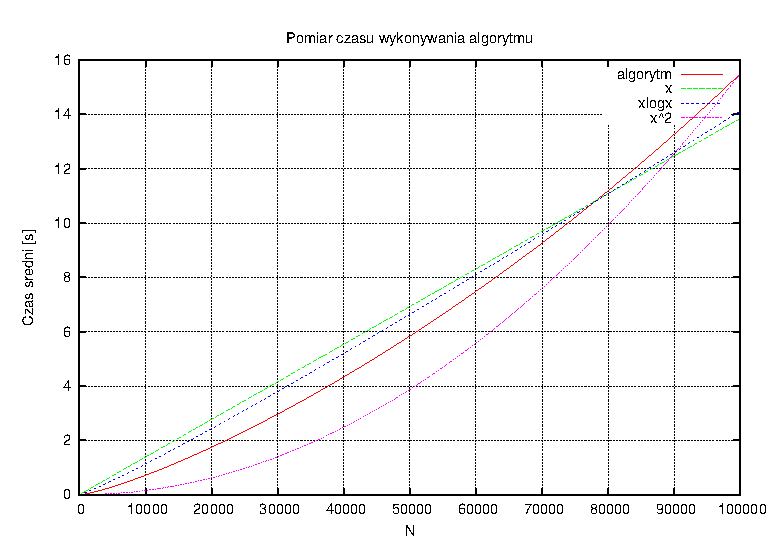
\includegraphics[width=1\textwidth]{../prj/wykres7.eps}
\caption{Wykres do tabeli nr 1}
\label{Wykres1}
\end{figure} 
\newpage
Na podstawie wykresu~\ref{Wykres1} i tabeli~\ref{tab1} złożoność obliczeniową algorytmu sortowania szybkiego dla danych posortowanych malejąco szacuje się na $ O(n^{2}) $.

 \item Heap-sort - dane malejące:
   
  \begin{table}[th]
  \centering
    \caption{Pomiar czasu sortowania przez kopcowanie dla danych posortowanych malejąco}

      \begin{tabular}{|l|l|l|}
	\hline
	N & czas & odchylenie \\
    \hline
 10 & 1.6762e-06 & 2.49005e-07\\
 \hline
100 & 4.6864e-06 & 4.41747e-07\\
\hline
1000 & 3.44455e-05 & 6.66292e-06\\
\hline
10000 & 0.000312184 & 3.15754e-05\\
\hline
50000 & 0.0015983 & 0.00015338\\
\hline
100000 & 0.0032386 & 0.000345748\\
\hline
    \end{tabular}
    \label{tab2}
    \end{table}
    \newpage
 \begin{figure}[!h]
\centering
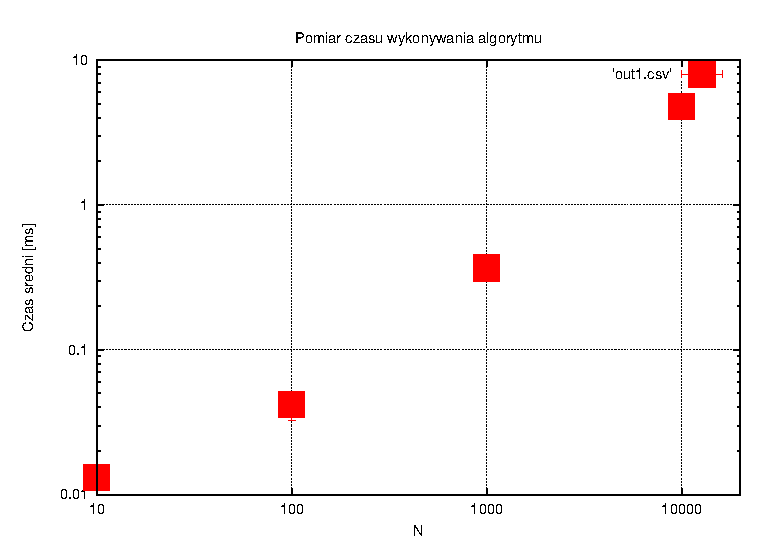
\includegraphics[width=1\textwidth]{../prj/wykres8.eps}
\caption{Wykres do tabeli nr 2}
\label{Wykres2}
\end{figure} 
Na podstawie wykresu~\ref{Wykres2} i tabeli~\ref{tab2} złożoność obliczeniową algorytmu sortowania przez kopcowanie dla danych posortowanych malejąco szacuje się na $ O(nlogn) $.
\item Mergesort - dane malejące:
  
  \begin{table}[th]
  \centering
    \caption{Pomiar czasu wykoniania sortowania przez scalanie dla danych posortowanych malejąco}

      \begin{tabular}{|l|l|l|}
	\hline
	N & czas & odchylenie \\
    \hline
  10 & 3.0871e-06 & 3.79339e-07\\
  \hline
100 & 4.37069e-05 & 4.27675e-06\\
\hline
1000 & 0.000739304 & 6.89142e-05\\
\hline
10000 & 0.00909738 & 0.000852001\\
\hline
50000 & 0.0590207 & 0.00537699\\
\hline
100000 & 0.128918 & 0.0118545\\
\hline
    \end{tabular}
    \label{tab3}
    \end{table}
\newpage
 \begin{figure}[!h]
\centering
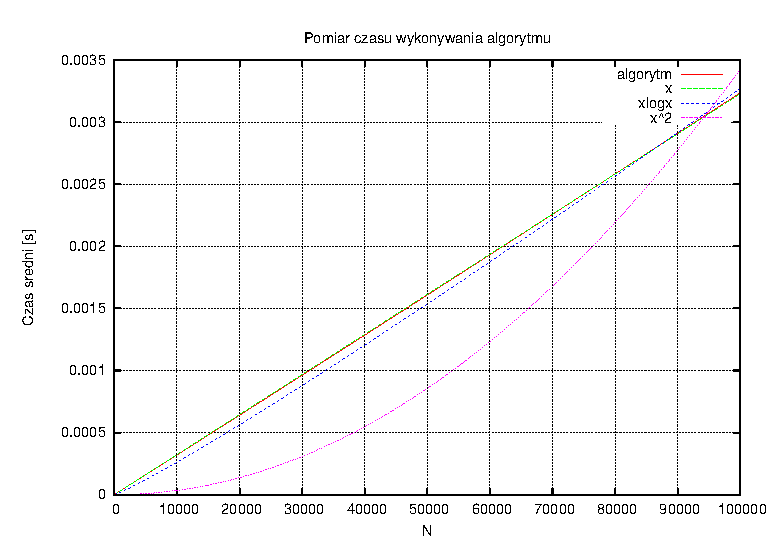
\includegraphics[width=1\textwidth]{../prj/wykres9.eps}
\caption{Wykres do tabeli nr 3}
\label{Wykres3}
\end{figure} 
Na podstawie wykresu~\ref{Wykres3} i tabeli~\ref{tab3} złożoność obliczeniową algorytmu sortowania przez scalanie dla danych posortowanych malejąco szacuje się na $ O(nlogn) $.
\item Quick-sort - dane rosnące:
  
  \begin{table}[th]
  \centering
    \caption{Pomiar czasu sortowania szybkiego dla danych posortowanych rosnąco}

      \begin{tabular}{|l|l|l|}
	\hline
	N & czas & odchylenie \\
    \hline
 10 & 2.165e-06 & 2.73961e-07\\
 \hline
100 & 2.21539e-05 & 2.6968e-06\\
\hline
1000 & 0.00161351 & 0.000150407\\
\hline
10000 & 0.162241 & 0.0210872\\
\hline
50000 & 4.1648 & 0.404208\\
\hline
100000 & 16.6305 & 1.54541\\

\hline
    \end{tabular}
    \label{tab4}
    \end{table}
    \newpage
 \begin{figure}[!h]
\centering
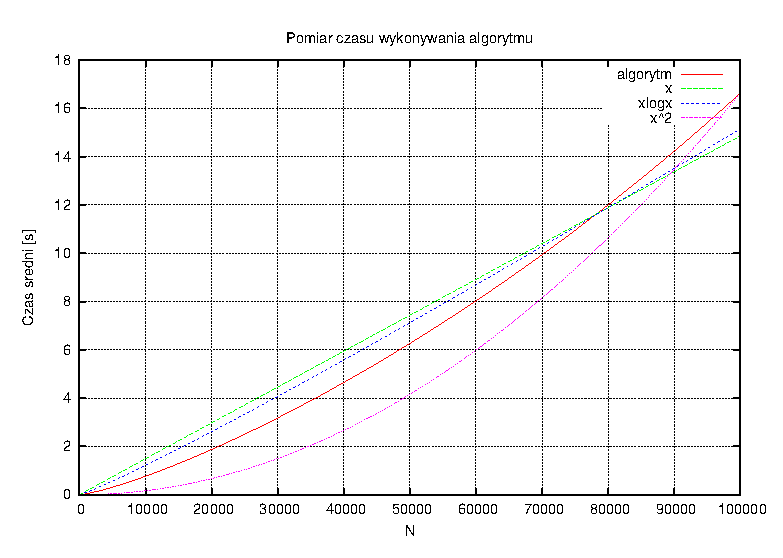
\includegraphics[width=1\textwidth]{../prj/wykres71.eps}
\caption{Wykres do tabeli nr 4}
\label{Wykres4}
\end{figure} 
Na podstawie wykresu~\ref{Wykres4} i tabeli~\ref{tab4} złożoność obliczeniową algorytmu sortowania szybkiego dla danych posortowanych rosnąco szacuje się na $ O(n^{2}) $.
 \item Heap-sort - dane rosnące:
   
  \begin{table}[th]
  \centering
    \caption{Pomiar czasu wykonania sortowania przez kopcowanie dla danych posortowanych rosnąco}

      \begin{tabular}{|l|l|l|}
	\hline
	N & czas & odchylenie \\
    \hline
  10 & 3.1777e-06 & 9.66352e-07\\
  \hline
100 & 1.41498e-05 & 1.37796e-06\\
\hline
1000 & 0.000129143 & 1.37132e-05\\
\hline
10000 & 0.00125259 & 0.000136966\\
\hline
50000 & 0.00610872 & 0.000647302\\
\hline
100000 & 0.0148653 & 0.00293036\\
\hline
    \end{tabular}
    \label{tab5}
    \end{table}
    \newpage
 \begin{figure}[!h]
\centering
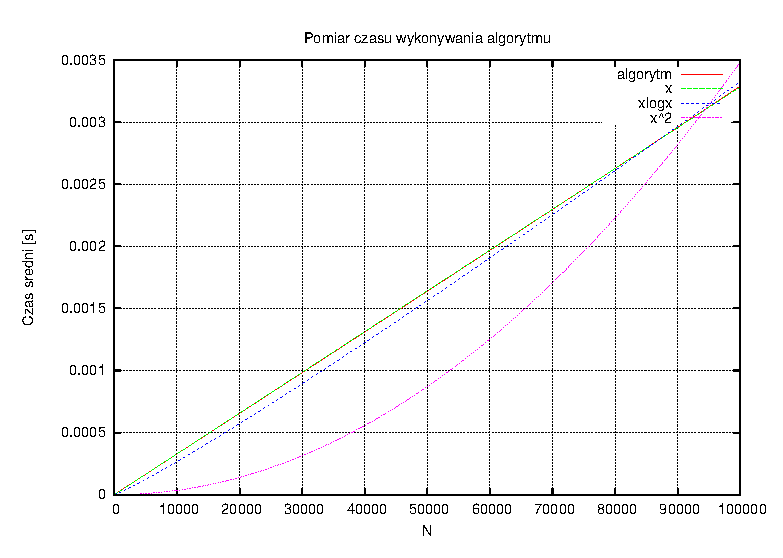
\includegraphics[width=1\textwidth]{../prj/wykres81.eps}
\caption{Wykres do tabeli nr 5}
\label{Wykres5}
\end{figure} 
Na podstawie wykresu~\ref{Wykres5} i tabeli~\ref{tab5} złożoność obliczeniową algorytmu sortowania przez kopcowanie dla danych posortowanych rosnącoo szacuje się na $ O(nlogn) $.
\item Mergesort - dane rosnące:
  
  \begin{table}[th]
  \centering
    \caption{Pomiar czasu sortowania przez scalanie dla danych posortowanych rosnąco}

      \begin{tabular}{|l|l|l|}
	\hline
	N & czas & odchylenie \\
    \hline
 10 & 1.7741e-06 & 2.50393e-07\\
 \hline
100 & 4.7632e-06 & 4.60575e-07\\
\hline
1000 & 3.37824e-05 & 3.05981e-06\\
\hline
10000 & 0.000329455 & 3.13672e-05\\
\hline
50000 & 0.00162924 & 0.000157049\\
\hline
100000 & 0.0032913 & 0.000301352\\
\hline
    \end{tabular}
    \label{tab6}
    \end{table}
\newpage
 \begin{figure}[!h]
\centering
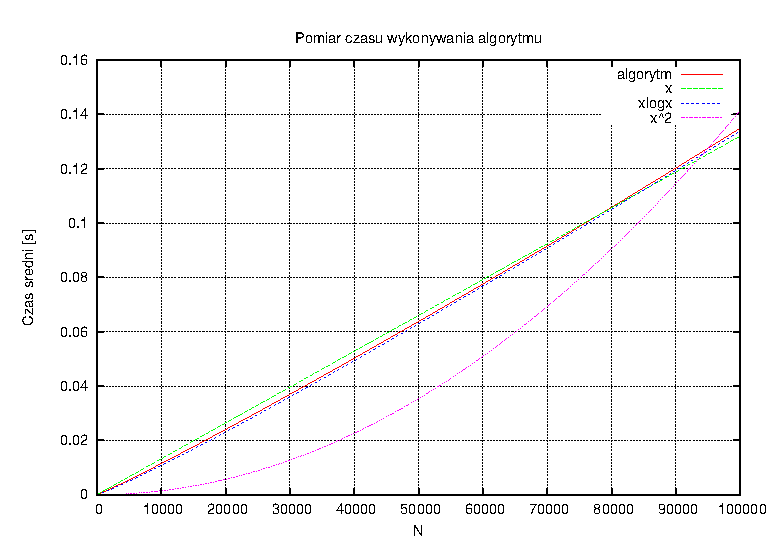
\includegraphics[width=1\textwidth]{../prj/wykres91.eps}
\caption{Wykres do tabeli nr 6}
\label{Wykres6}
\end{figure} 

Na podstawie wykresu~\ref{Wykres6} i tabeli~\ref{tab6} złożoność obliczeniową algorytmu sortowania przez scalanie dla danych posortowanych rosnąco szacuje się na $ O(nlogn) $.
\item Quick-sort - dane przypadkowe:
  
  \begin{table}[th]
  \centering
    \caption{Pomiar czasu sortowania szybkiego danych ułożonych w losowej kolejności}

      \begin{tabular}{|l|l|l|}
	\hline
	N & czas & odchylenie \\
    \hline
 10 & 2.2279e-06 & 3.13207e-07\\
 \hline
100 & 1.4527e-05 & 1.44116e-06\\
\hline
1000 & 0.000188593 & 1.76021e-05\\
\hline
10000 & 0.00265908 & 0.000800968\\
\hline
500000 & 0.182986 & 0.0242359\\
\hline
1000000 & 0.340734 & 0.0328892\\
\hline
    \end{tabular}
    \label{tab7}
    \end{table}
    \newpage
 \begin{figure}[!h]
\centering
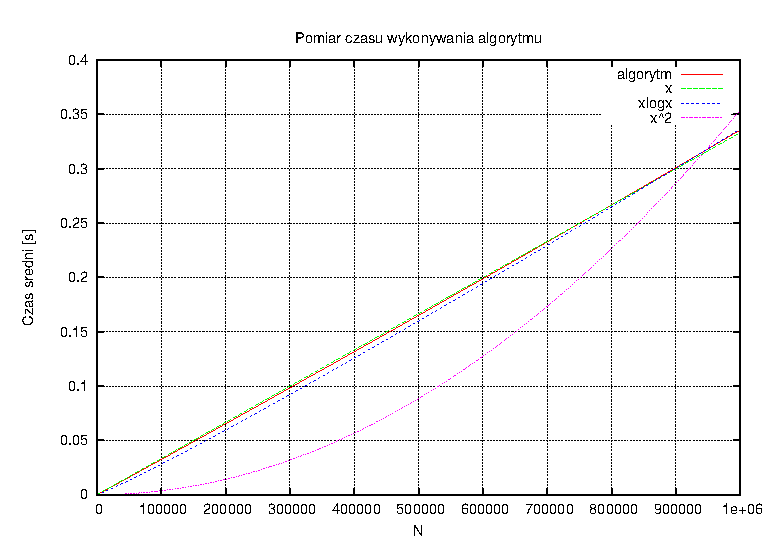
\includegraphics[width=1\textwidth]{../prj/wykres72.eps}
\caption{Wykres do tabeli nr }7
\label{Wykres7}
\end{figure} 
Na podstawie wykresu~\ref{Wykres7} i tabeli~\ref{tab7} złożoność obliczeniową algorytmu sortowania szybkiego dla danych ułożonych losowo szacuje się na $ O(nlogn) $.
 \item Heap-sort - dane przypadkowe:
   
  \begin{table}[th]
  \centering
    \caption{Pomiar czas sortowania szybkiego danych ułożonych przypadkowo}

      \begin{tabular}{|l|l|l|}
	\hline
	N & czas & odchylenie \\
    \hline
 10 & 1.8508e-06 & 2.27902e-07\\
 \hline
100 & 4.8819e-06 & 4.74368e-07\\
\hline
1000 & 3.432e-05 & 3.1194e-06\\
\hline
10000 & 0.000334107 & 3.23179e-05\\
\hline
500000 & 0.0244684 & 0.00483988\\
\hline
1000000 & 0.0372819 & 0.00902984\\
\hline
    \end{tabular}
    \label{tab8}
    \end{table}
    \newpage
 \begin{figure}[!h]
\centering
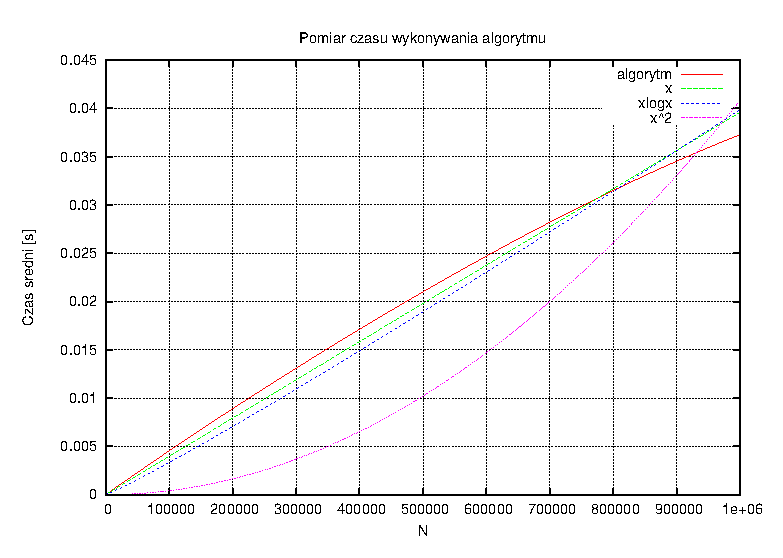
\includegraphics[width=1\textwidth]{../prj/wykres82.eps}
\caption{Wykres do tabeli nr 8}
\label{Wykres8}
\end{figure} 
Na podstawie wykresu~\ref{Wykres8} i tabeli~\ref{tab8} złożoność obliczeniową algorytmu sortowania przez kopcowanie szybkiego dla danych ułożonych losowo szacuje się na $ O(nlogn) $.
\item Mergesort - dane przypadkowe:
  
  \begin{table}[th]
  \centering
    \caption{Pomiar sortowania przez scalanie danych ułożonych przypadkowo}

      \begin{tabular}{|l|l|l|}
	\hline
	N & czas & odchylenie \\
    \hline
 10 & 2.9822e-06 & 3.79038e-07\\
 \hline
100 & 4.42445e-05 & 4.52298e-06\\
\hline
1000 & 0.000785393 & 8.62454e-05\\
\hline
10000 & 0.00955412 & 0.000909519\\
\hline
500000 & 0.883084 & 0.0849108\\
\hline
1000000 & 1.87052 & 0.166319\\

\hline
    \end{tabular}
    \label{tab9}
    \end{table}
\newpage
 \begin{figure}[!h]
\centering
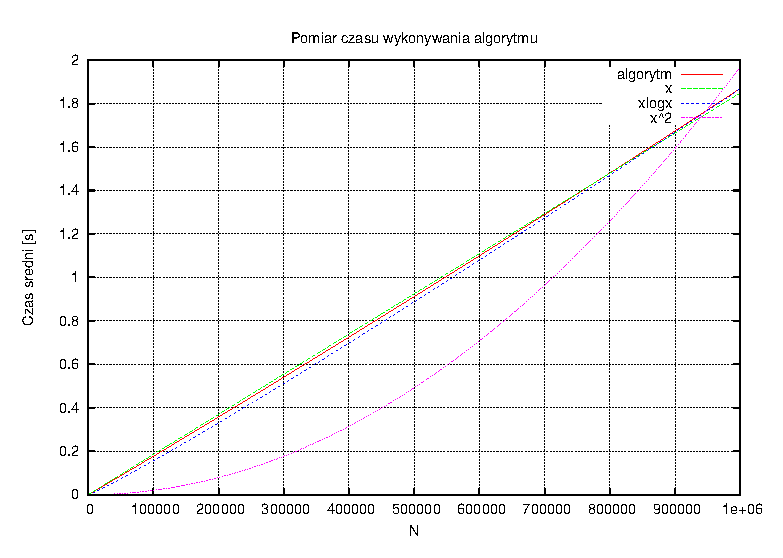
\includegraphics[width=1\textwidth]{../prj/wykres92.eps}
\caption{Wykres do tabeli nr 9}
\label{Wykres9}
\end{figure} 
Na podstawie wykresu~\ref{Wykres9} i tabeli~\ref{tab9} złożoność obliczeniową algorytmu sortowania przez scalanie dla danych ułożonych losowo szacuje się na $ O(nlogn) $.
\item Quick-sort - dane posortowane z usprawnieniem algorytmu (wybieranie środkowego elementu):
  
  \begin{table}[th]
  \centering
    \caption{Pomiar sortowania szybkiego danych uprzednio posortowanych(ze środkowym elementem pełniącym rolę pivota)}

      \begin{tabular}{|l|l|l|}
	\hline
	N & czas & odchylenie \\
    \hline
 10 & 1.8649e-06 & 2.82212e-07\\
 \hline
100 & 6.0485e-06 & 5.95969e-07\\
\hline
1000 & 5.18922e-05 & 5.21905e-06\\
\hline
10000 & 0.000637951 & 5.80617e-05\\
\hline
500000 & 0.0425858 & 0.0045352\\
\hline
1000000 & 0.0935673 & 0.0140937\\

\hline
    \end{tabular}
    \label{tab10}
    \end{table}
    \newpage
 \begin{figure}[!h]
\centering
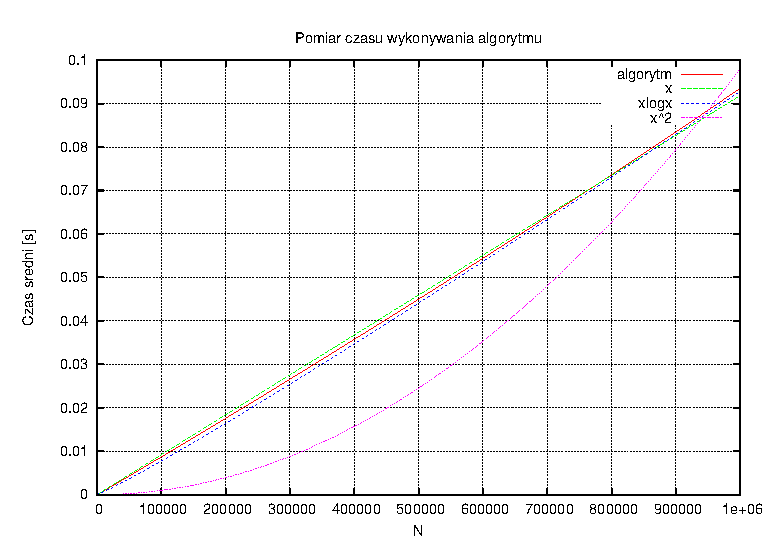
\includegraphics[width=1\textwidth]{../prj/wykres73.eps}
\caption{Wykres do tabeli nr 10}
\label{Wykres10}
\end{figure} 
Na podstawie wykresu~\ref{Wykres10} i tabeli~\ref{tab10} złożoność obliczeniową algorytmu sortowania szybkiego dla danych ułożonych losowo i po usprawnieniu algorytmu szacuje się na $ O(nlogn) $.
\newpage
\section{Wnioski}
\begin{itemize}
 \item Sortowanie szybkie, spośród powyższych, okazało się najłatwiejsze w implementacji.
 \item Złożoność obliczeniową powyższych algorytmów szacuje się na $ O(n logn) $
 \item Algorytm sortowania szybkiego okazał się najszybszy, co nie oznacza, że jest on niezawodny. Istnieje taka możliwość, gdzie złożoność obliczeniowa 
 algorytmu sortowania szybkiego wynosi $ O(n^{2}) $. Dotyczy ona np. tablicy uprzednio posortowanej. Gdy takie sytuacje miałyby miejsce dość często, warto wówczas usprawnić algorytm sortowania szybkiego. Jednym z rozwiaząń, użytym w badaniach, był zabieg 
 polegający na wybieraniu środkowego indeksu tablicy, jako elementu słuzącego do partycjonowania całości. Nie jest to rozwiązanie idealne, aczkolwiek znacząco usprawnia algorytm i chroni przed 
 danymi posortowanymi. Inną metodą może być też poszukiwanie mediany; znajdowanie mediany całego zbioru cechuje się dużą złożonością, dlatego też 
 wybiera się losowe elementy tablicy i to z ich mediany ustala się element rozdzielający, co zapobiega trafieniu na największy element.
 \item Algorytmy sortowania stogowego i sortowania przez scalanie mają gwarantowaną złozoność niezależnie od danych wejściowych, więc
 są dobrą alternatywą dla algorytmu quicksort.
\end{itemize}


\end{enumerate}
\end{document}
